% super simple template for automated 2021 ADASS manuscript generation from the registration entry
% place this file in your ADASS2021_author_template directory together with your makedefs file
%
% Only few comments here, see the ADASS_template.tex for a more fully commented version, and
% ManuscriptInstructions.pdf if you need more background, and if you even need more, APS's own
% manual2010.pdf has it all!

% Version 5-oct-2021 (Peter Teuben & Benjamin Hugo)

\documentclass[11pt,twoside]{article}
\usepackage{asp2014}

\aspSuppressVolSlug
\resetcounters

\bibliographystyle{asp2014}

\markboth{Rodriguez et al.}{The SIMPLE Archive}
% remove/add as you need

\begin{document}

\title{The SIMPLE Archive}

% full name: David Rodriguez
\author{David~Rodriguez$^1$, Kelle~Cruz$^2$, Will~Cooper$^3$, Niall~Whiteford$^4$, Clemence~Fontanive$^5$, 
Ella~Hort$^6$, Sherelyn~Alejandro$^2$, Robert~Blackwell$^7$, Daniel~Terach$^8$}
\affil{$^1$Space Telescope Science Institute, Baltimore, MD, USA; \email{drodriguez@stsci.edu}}
\affil{$^2$CUNY Hunter College, New York, NY, USA}
\affil{$^3$University of Hertfordshire, Hertfordshire, United Kingdom}
\affil{$^4$University of Edinburgh, Edinburgh, Scotland, United Kingdom}
\affil{$^5$CSH, University of Bern, Bern, Switzerland}
\affil{$^6$Pomona College, Claremont, CA, USA}
\affil{$^7$Flatiron Institute, New York, NY, USA}
\affil{$^8$Pace University, New York, NY, USA}
% remove/add as you need

% remove/add authors as you need
\paperauthor{David~Rodriguez}{drodriguez@stsci.edu}{0000-0003-1286-5231}{Space Telescope Science Institute}{}{Baltimore}{MD}{}{USA}
\paperauthor{Kelle~Cruz}{}{}{CUNY Hunter College}{}{New York}{NY}{}{USA}
\paperauthor{Will~Cooper}{}{}{University of Hertfordshire}{}{Hertfordshire}{}{}{United Kingdom}
\paperauthor{Niall~Whiteford}{}{}{University of Edinburgh}{}{Edinburgh}{Scotland}{}{United Kingdom}
\paperauthor{Clemence~Fontanive}{}{}{CSH, University of Bern}{}{Bern}{}{}{Switzerland}
\paperauthor{Ella~Hort}{}{}{Pomona College}{}{Claremont}{CA}{}{USA}
\paperauthor{Sherelyn~Alehandro}{}{}{CUNY Hunter Colleg}{}{New York}{NY}{}{USA}
\paperauthor{Robert~Blackwell}{}{}{Flatiron Institute}{}{New York}{NY}{}{USA}
\paperauthor{Daniel~Terach}{}{}{Pace University}{}{New York}{NY}{}{USA}
% \paperauthor{Name}{Email}{ORCID}{college}{Author2 Department}{City}{State}{Postal Code}{Country}

% remove/add as you need

% leave these next few aindex lines commented for the editors to enable them. Use Aindex.py to generate them for yourself.
% first presenting author should be the first entry for bold-facing the author index page-reference
%\aindex{Rodriguez,~D.}
%\aindex{Author2,~S.}
% remove/add as you need

% leave the ssindex lines commented for the editors to enable them, use Index.py to suggest yours
%\ssindex{FOOBAR!conference!ADASS 2020}
%\ssindex{FOOBAR!organisations!ASP}

% leave the ooindex lines commented for the editors to enable them, use ascl.py to suggest yours
%\ooindex{FOOBAR, ascl:1101.010}
  
\begin{abstract}

We present the SIMPLE Archive alongside its database management tool, AstrodbKit2. SIMPLE is an archive of low mass stars, brown dwarfs, and exoplanets driven by community curation and review using GitHub. SIMPLE relies on AstrodbKit2 to convert back and forth from a document-store model of the database, to a more standard relational database that can be used with established packages like SQLAlchemy. In this poster, we present the architecture of the SIMPLE database and how using AstrodbKit2 facilitates a git workflow for reviewing and approving database modifications.

SIMPLE is available at https://github.com/SIMPLE-AstroDB/SIMPLE-db 

AstrodbKit2 is available at https://github.com/dr-rodriguez/AstrodbKit2
  
\end{abstract}

\section{SIMPLE}

SIMPLE is an archive of low mass stars, brown dwarfs, and exoplanets. The vision behind SIMPLE is that of a community-driven archive were individual contributors help grow the knowledge base of these objects. 
SIMPLE contains a variety of data and supporting metadata for these low mass objects, but serves as an example that can be adapted to other fields of study, such as extragalactic or supernova archives. 
SIMPLE strives to represent each individual source as a consistent object that can be understood and referenced by others during the community review process. To that end, supporting software (AstrodbKit2) had to be created to facility this workflow.

\section{AstrodbKit2}

AstrodbKit2 is a Python package that uses SQLAlchemy to create and connect to a variety of relational databases (eg, SQLite, Postgres, MSSQL, etc). Tables in AstrodbKit2 are organized into two types: \textit{Object} tables, which have one-to-many relationships to a single primary object table (ie, Sources in the SIMPLE database); and \textit{Reference} tables, which have many-to-many relationships against the object tables and are used to store lookup information like publications, telescopes, or instruments. The SIMPLE Archive gathers measurements for low mass objects into a variety of tables all associated to the primary Sources table by their source name. Object tables in SIMPLE include Photometry, Proper Motions, Radial Velocities, and Spectra; Reference tables include Publications, Telescopes, and Instruments.

Using AstrodbKit2, we can convert the SIMPLE database from a document store mode, where individual Sources are stored as separate JSON files (which can in turn be loaded into NoSQL databases like MongoDB), to a relational database such as SQLite or Postgres that can be accessed with standard tools (see Figure~\ref{fig:astrodbkit2}). JSON files, such as the example in Figure~\ref{fig:json} serve as the definitive copy of the database for purposes of version control.

\begin{figure}
    \centering
    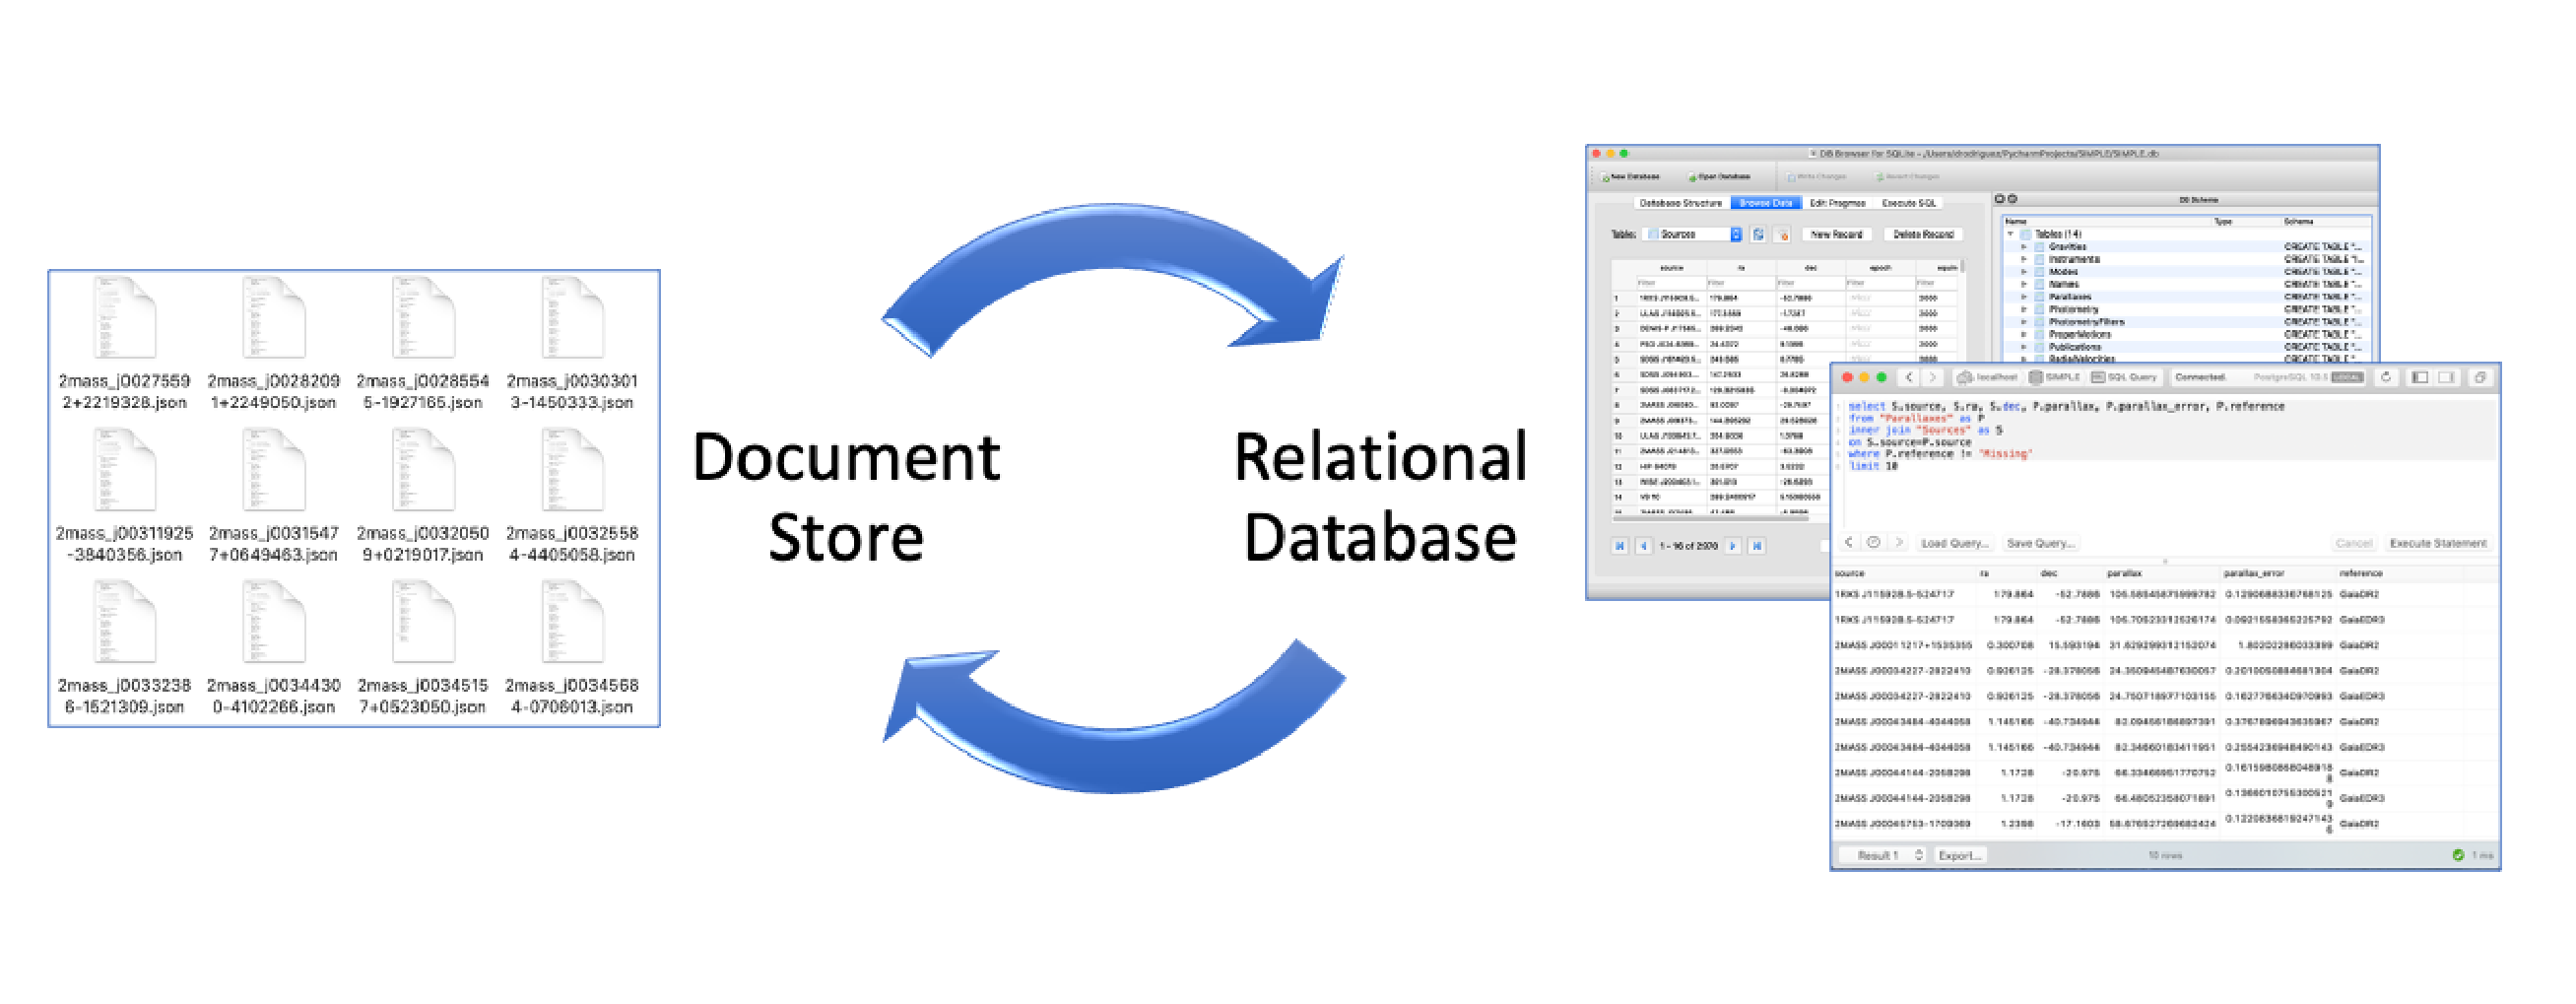
\includegraphics[width=\textwidth]{X0-012_f1.eps}
    \caption{AstrodbKit2 can convert a database from a document store representation (eg, a list of JSON files) to a relational database (eg, SQLite, Postgres, etc).}
    \label{fig:astrodbkit2}
\end{figure}

\section{Collaborative Workflow}

By exporting a database to a JSON document store, we can use git and GitHub to handle version control for our database as well as curate commits via pull requests. 
An individual user may contain their own copy of SIMPLE, or any other database supported by AstrodbKit2. They may make changes in their local branch and push to their copy on GitHub. By issuing a pull request they request their changes be adopted into the main branch of the database. Because the database is stored as individual JSON documents, reviewers can see exactly which objects have been updated and can comment on the changes if needed. By using a simple to read format, we benefit from a clear picture of the changes in a pull request. 

As part of the pull request process, automatic tests are run to verify the integrity of the database. This ensures no changes took place that break the functionality of the database. Finally, when the pull request is accepted, additional automated tasks can be performed to regenerate the database and push it to external users of the database, such as a graphical user interface.


\begin{figure}
    \centering
    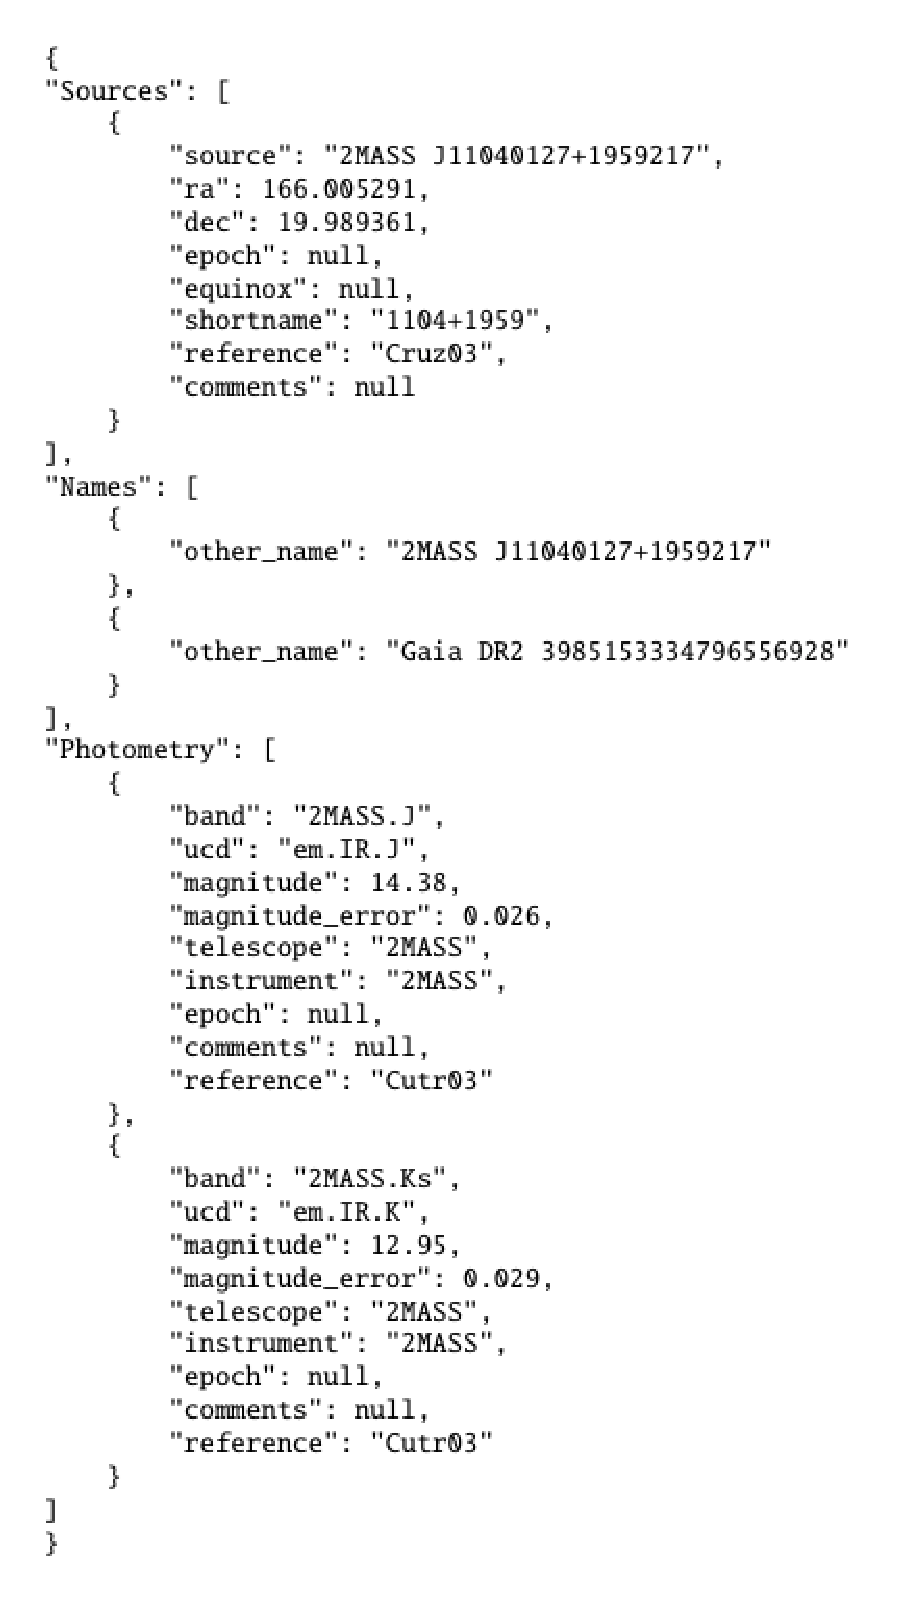
\includegraphics[height=0.9\textheight]{X0-012_f2.eps}
    \caption{Trimmed JSON document for a source in the SIMPLE database}
    \label{fig:json}
\end{figure}

% For example in \citet{PID_adassxxx} it was shown that ...


% \bibliography{X0-012}


% if we have space left, we might add a conference photograph here. Leave commented for now.
% \bookpartphoto[width=1.0\textwidth]{foobar.eps}{FooBar Photo (Photo: Any Photographer)}


\end{document}

